% !TeX root = main.tex
\chapterimage{chapter-05-rappresentazione-informazione.jpg}
\chapter{Rappresentazione dell'informazione}\label{capitolo-5-rappresentazione-dellinformazione}

L'essere umano ha sempre cercato modi per codificare le informazioni, cioè per tradurle in simboli che possano essere conservati, condivisi e compresi da altri. Molti di questi sistemi fanno parte della nostra vita quotidiana e li usiamo senza nemmeno pensarci:

\begin{itemize}
\item
  l'alfabeto per rappresentare i suoni delle parole attraverso lettere scritte;
\item
  le note musicali per rappresentare i suoni di una melodia su un pentagramma;
\item
  le cifre per rappresentare quantità e numeri;
\item
  i cartelli stradali per rappresentare regole di comportamento;
\item
  più recentemente, gli emoji per rappresentare emozioni.
\end{itemize}

Questi sono tutti esempi di rappresentazioni: modi convenzionali per trasformare qualcosa di complesso (un suono, un'immagine, un luogo, un'azione) in un insieme di simboli che possiamo leggere, interpretare e ricostruire.

In informatica, il principio è lo stesso: vengono prima scelti dei dati da usare per parlare di un'informazione (un testo, un disegno, un suono, un video); poi, i dati scelti vengono codificati con simboli seguendo regole precise. Si può anche percorrere il processo contrario, cioè quello della decodifica, che dalla rappresentazione dei dati permette di ricostruire l'informazione. Il processo di codifica e decodifica permette di memorizzare, trasmettere e ricostruire in modo affidabile l'informazione per un esecutore automatico; per le persone, l'interpretazione dipende comunque dal contesto e dalle conoscenze pregresse.

A seconda della rappresentazione scelta, i dati potranno essere più o meno facili da elaborare da una macchina, occupare più o meno spazio, essere più o meno veloci da leggere o da scrivere.

Le attività di questa sezione aiuteranno alunni e alunne a sperimentare in modo concreto queste idee: esploreranno diversi modi per descrivere la stessa cosa e si confronteranno con i processi di codifica e decodifica.

\section{Traguardi e obiettivi generali }\label{traguardi-e-obiettivi-generali-2}

\begin{itemize}
\item
  Descrivere a parole il funzionamento di semplici sistemi di codifica e decodifica.
\item
  Applicare correttamente le regole di un sistema di codifica dato per: decodificare immagini in \emph{pixel art}; ricostruire messaggi a partire da sequenze di simboli.
\item
  Codificare immagini o messaggi in una rappresentazione simbolica.
\item
  Confrontare e valutare diversi sistemi di codifica in termini di univocità e costo.
\item
  Confrontare diverse rappresentazioni della stessa informazione.
\item
  Individuare e correggere ambiguità o errori nel processo di codifica e/o decodifica (debugging).
\end{itemize}

\section{Prerequisiti }\label{prerequisiti-2}

Le attività proposte non richiedono particolari conoscenze informatiche pregresse. È sufficiente che bambini e bambine:

\begin{itemize}
\item
  sappiano seguire consegne orali e scritte e riconoscano alcune parole o frasi brevi (per le attività sui messaggi di Alice e Bob);
\item
  abbiano familiarità con griglie, con il riconoscimento di una casella come incrocio tra righe e colonne (ad esempio, hanno giocato almeno una volta a battaglia navale), e con i numeri naturali (per contare caselle, leggere coordinate);
\item
  riconoscano e utilizzino alcuni colori per completare disegni su una griglia.
\end{itemize}

\section{Contenuti, in breve }\label{contenuti-in-breve-2}

Questo capitolo propone tre attività, a difficoltà crescente, in cui studenti e studentesse imparano a decodificare prima e rappresentare poi informazioni usando codifiche condivise. Le attività li guidano gradualmente dal ruolo di esecutore, che interpreta e applica una codifica data, al ruolo di programmatore, che crea e comunica una propria codifica affinché altri possano ricostruire correttamente le informazioni.

Per rendere l'esperienza più coinvolgente, è possibile inserire ogni attività in un contesto narrativo o ludico (messaggi segreti, mappe del tesoro, disegni nascosti, e così via).

\textbf{Attività 1 -- Capire il sistema di codifica}: bambini e bambine hanno a disposizione alcune immagini su griglie di piccole dimensioni (ad esempio \(2 \times 2\)) associate a un sistema di codifica e, lavorando per ipotesi e confronti, ricostruiscono le regole del sistema di codifica (ad esempio l'ordine di lettura, il significato di eventuali simboli numerici o alfabetici presenti, associazione tra simboli e dati scelti per descrivere l'immagine).

\textbf{Attività 2 -- Pixel art}: bambini e bambine lavorano con immagini in pixel art su griglie (fino a \(10 \times 10\)) per sperimentare due ruoli: l'\,``esecutore'', che decodifica una codifica data per ricostruire un disegno, e soprattutto il ``programmatore'', che scrive la codifica di un'immagine (inventata o assegnata) seguendo regole e simboli condivisi.

\textbf{Attività 3 -- Luci di Natale}: bambini e bambine prima confrontano diversi codici per rappresentare un insieme di messaggi per trovare quelli che permettono di capirsi sempre e quali sono più costosi. In una seconda parte dell'attività, progettano un nuovo codice condiviso che rispetti alcuni vincoli di brevità.

\section{Modalità di lavoro }\label{modalituxe0-di-lavoro-2}

Tutte le attività che seguono possono essere svolte in classe.

\begin{itemize}
\item
  Si alterneranno fasi di lavoro a coppie con momenti di confronto collettivo o a piccoli gruppi e sarà importante dare spazio sia alla fase esecutiva (seguire una codifica) sia a quella creativa (progettare una propria codifica), valorizzando le differenze tra le soluzioni.
\item
  Sarà importante osservare lo svolgimento delle varie attività tenendo traccia delle parole e delle produzioni di alunni e alunne (ad esempio, fornendo schede strutturate per scrivere o disegnare, ma anche scattando foto alle loro produzioni) da usare a supporto di discussioni collettive.
\end{itemize}

Le Attività 1 e 2 propongono di svolgere codifica e decodifica di immagini utilizzando due diversi sistemi di codifica: per righe e per coordinate.

\subsubsection{Codifica per righe}

Questo sistema di codifica funziona così: la griglia viene letta una riga alla volta da sinistra verso destra. Per ogni riga, la figura non viene descritta quadretto per quadretto, ma come una sequenza di caselle tutte dello stesso colore. Ogni sequenza di caselle è scritta con:

\begin{itemize}
\item
  un numero, che indica quanti quadretti consecutivi vanno considerati;
\item
  una lettera, che indica il colore (legenda: B = bianco, A = arancione, M = marrone, N = nero).
\end{itemize}

Di seguito un esempio, con la prima riga già colorata:

\begin{center}
\begin{minipage}{\linewidth}
\centering
\renewcommand{\arraystretch}{1.4}
\begin{minipage}[c]{0.36\linewidth}
\centering
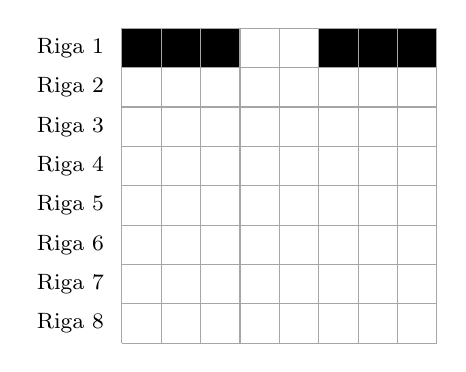
\begin{tikzpicture}[scale=0.5]
	\foreach \r in {1,...,8} \node[left=3pt,font=\footnotesize] at (0,8.5-\r) {Riga \r};
	\fill[black] (0,7) rectangle (3,8);
	\fill[black] (5,7) rectangle (8,8);
	\draw[gray!70,thin] (0,0) grid (8,8);
\end{tikzpicture}
\end{minipage}\hfill
\begin{minipage}[c]{0.62\linewidth}
\begin{tabular}{|>{\raggedright\arraybackslash}m{\dimexpr\linewidth-2\tabcolsep-2\arrayrulewidth\relax}|}
\hline
\multicolumn{1}{|c|}{\cellcolor{black!15}\textbf{REGOLE DI COLORAZIONE}} \\
\hline
\cbxv{} \textbf{Riga 1}: 3N - 2B - 3N \\
\hline
\cbx{} \textbf{Riga 2}: 1N - 1B - 1M - 2A - 1M - 1B - 1N \\
\hline
\cbx{} \textbf{Riga 3}: 1N - 1M - 4A - 1M - 1N \\
\hline
\cbx{} \textbf{Riga 4}: 2A - 1B - 2A - 1B - 2A \\
\hline
\cbx{} \textbf{Riga 5}: 1A - 1B - 1N - 2A - 1N - 1B - 1A \\
\hline
\cbx{} \textbf{Riga 6}: 1N - 1B - 1A - 2N - 1A - 1B - 1N \\
\hline
\cbx{} \textbf{Riga 7}: 1B - 1N - 4B - 1N - 1B \\
\hline
\cbx{} \textbf{Riga 8}: 2B - 4N - 2B \\
\hline
\end{tabular}
\end{minipage}
\par\medskip
\begin{tabular}{|*{4}{>{\centering\arraybackslash}m{\dimexpr0.25\linewidth-2\tabcolsep-5\arrayrulewidth/4\relax}|}}
\hline
\multicolumn{4}{|c|}{\cellcolor{black!15}\textbf{LEGENDA COLORI}} \\
\hline
\tikz[baseline=0.4ex]\draw[gray!70,fill=white] (0,0) rectangle (0.8em,0.8em); B = bianco &
\tikz[baseline=0.4ex]\draw[gray!70,fill=codArancione] (0,0) rectangle (0.8em,0.8em); A = arancione &
\tikz[baseline=0.4ex]\draw[gray!70,fill=codMarrone] (0,0) rectangle (0.8em,0.8em); M = marrone &
\tikz[baseline=0.4ex]\draw[gray!70,fill=black] (0,0) rectangle (0.8em,0.8em); N = nero \\
\hline
\end{tabular}
\end{minipage}
\end{center}

Ad esempio, ``3N - 2B - 3N'' per la riga 1 significa che, in quella riga, ci sono nell'ordine: 3 quadretti neri, poi 2 bianchi, poi 3 neri.

\subsubsection{Codifica per coordinate}


Questo sistema di codifica funziona così: la griglia è formata da righe indicate con le lettere (A, B, C, \ldots, L) e colonne indicate con i numeri (1, 2, 3, \ldots, 10). Ad ogni casella dell'immagine, viene associata una coppia ordinata (numero, lettera) in cui il numero indica la colonna della casella, mentre la lettera indica la riga della casella.

Per decodificare l'immagine, si prende un colore alla volta tra quelli indicati e si colorano le celle che corrispondono alle coordinate nell'elenco corrispondente.

Di seguito un esempio.


\begin{center}
\begin{minipage}{\linewidth}
\centering
\renewcommand{\arraystretch}{1.2}
\newcommand{\pixelcoordinata}[1]{\mbox{\cbx{} (#1)}}
\begin{tikzpicture}[scale=0.6]
  \foreach[count=\i] \l in {A,B,C,D,E,F,G,H,I,L}
    \node[left=4pt,font=\small] at (0,10.5-\i) {\l};
  \foreach \c in {1,...,10}
    \node[above=3pt,font=\small] at (\c-0.5,10) {\c};
  \fill[codAzzurro] (1,9) rectangle (2,10);
  \fill[codAzzurro] (8,9) rectangle (9,10);
  \draw[gray!70,thin] (0,0) grid (10,10);
\end{tikzpicture}
\par\medskip
\begin{minipage}[t]{0.49\linewidth}
\vspace{0pt}
\begin{tabular}{|>{\raggedright\arraybackslash}m{\dimexpr\linewidth-2\tabcolsep-2\arrayrulewidth\relax}|}
\hline
\multicolumn{1}{|c|}{\cellcolor{codViola}\textcolor{white}{\textbf{VIOLA}}} \\
\hline
\pixelcoordinata{4, B}\quad \pixelcoordinata{6, B}\quad \pixelcoordinata{7, B} \\[\arrayrulewidth]
\pixelcoordinata{3, C}\quad \pixelcoordinata{4, C}\quad \pixelcoordinata{5, C}\newline
\pixelcoordinata{6, C}\quad \pixelcoordinata{8, C} \\[\arrayrulewidth]
\pixelcoordinata{2, D}\quad \pixelcoordinata{3, D}\quad \pixelcoordinata{4, D}\quad \pixelcoordinata{6, D}\newline
\pixelcoordinata{7, D}\quad \pixelcoordinata{8, D}\quad \pixelcoordinata{9, D} \\[\arrayrulewidth]
\pixelcoordinata{2, E}\quad \pixelcoordinata{5, E}\quad \pixelcoordinata{6, E}\quad \pixelcoordinata{9, E} \\[\arrayrulewidth]
\pixelcoordinata{2, F}\quad \pixelcoordinata{5, F}\quad \pixelcoordinata{6, F}\quad \pixelcoordinata{9, F} \\[\arrayrulewidth]
\pixelcoordinata{3, G}\quad \pixelcoordinata{4, G}\quad \pixelcoordinata{7, G}\quad \pixelcoordinata{8, G} \\[\arrayrulewidth]
\pixelcoordinata{2, H}\quad \pixelcoordinata{3, H}\quad \pixelcoordinata{4, H}\quad \pixelcoordinata{5, H}\newline
\pixelcoordinata{6, H}\quad \pixelcoordinata{7, H}\quad \pixelcoordinata{8, H}\quad \pixelcoordinata{9, H} \\[\arrayrulewidth]
\pixelcoordinata{1, I}\quad \pixelcoordinata{2, I}\quad \pixelcoordinata{4, I}\quad \pixelcoordinata{5, I}\newline
\pixelcoordinata{6, I}\quad \pixelcoordinata{7, I}\quad \pixelcoordinata{9, I}\quad \pixelcoordinata{10, I} \\[\arrayrulewidth]
\pixelcoordinata{1, L}\quad \pixelcoordinata{4, L}\quad \pixelcoordinata{7, L}\quad \pixelcoordinata{10, L} \\
\hline
\end{tabular}
\end{minipage}\hfill
\begin{minipage}[t]{0.49\linewidth}
\vspace{0pt}
\begin{tabular}{|>{\raggedright\arraybackslash}m{\dimexpr\linewidth-2\tabcolsep-2\arrayrulewidth\relax}|}
\hline
\multicolumn{1}{|c|}{\cellcolor{black}\textcolor{white}{\textbf{NERO}}} \\
\hline
\pixelcoordinata{4, E}\quad \pixelcoordinata{8, E} \\[\arrayrulewidth]
\pixelcoordinata{3, F}\quad \pixelcoordinata{4, F}\quad \pixelcoordinata{7, F}\quad \pixelcoordinata{8, F} \\[\arrayrulewidth]
\pixelcoordinata{5, G}\quad \pixelcoordinata{6, G} \\
\hline
\end{tabular}
\par\medskip
\begin{tabular}{|>{\raggedright\arraybackslash}m{\dimexpr\linewidth-2\tabcolsep-2\arrayrulewidth\relax}|}
\hline
\multicolumn{1}{|c|}{\cellcolor{codRosa}\textbf{ROSA}} \\
\hline
\pixelcoordinata{2, G}\quad \pixelcoordinata{9, G} \\
\hline
\end{tabular}
\par\medskip
\begin{tabular}{|>{\raggedright\arraybackslash}m{\dimexpr\linewidth-2\tabcolsep-2\arrayrulewidth\relax}|}
\hline
\multicolumn{1}{|c|}{\cellcolor{codAzzurro}\textbf{AZZURRO}} \\
\hline
\mbox{\cbxv{} (2, A)}\quad \mbox{\cbxv{} (9, A)} \\[\arrayrulewidth]
\pixelcoordinata{5, B} \\[\arrayrulewidth]
\pixelcoordinata{1, C}\quad \pixelcoordinata{7, C}\quad \pixelcoordinata{10, C} \\[\arrayrulewidth]
\pixelcoordinata{5, D} \\
\hline
\end{tabular}
\end{minipage}
\end{minipage}
\end{center}

Ad esempio, nella sezione \emph{AZZURRO}, la coppia \textbf{(2, A)} significa: ``colora di azzurro la casella che si trova nella colonna 2, riga A''.

\section{Attività 1: capire il sistema di codifica}

\ruoliattivita{\ruoloProgrammatore\quad\ruoloEsecutore}

Data un'informazione, una scelta di dati ad essa associati e un sistema di codifica per rappresentare tali dati, il primo passo è quello di capire come funziona quel sistema di codifica.

\subsection{Preparazione }\label{preparazione-4}

\begin{itemize}
\item
  Stampare e ritagliare schede con varie informazioni rappresentate da dati codificati secondo un certo sistema di codifica da analizzare (o eventualmente completare/creare).
\item
  Post-it (per disegnare o scrivere numeri, parole chiave).
\end{itemize}

\subsection{Obiettivo }\label{obiettivo-4}


Rendere esplicito il collegamento tra i simboli usati nella codifica e i dati scelti per parlare di un'informazione.

\subsection{Descrizione}


Si predispongono una serie di schede, ciascuna contenente delle immagini che consistono in una griglia 2x2 con alcune caselle colorate con diverse combinazioni di colori e, di fianco, una sequenza di simboli che rappresenta la codifica simbolica di quell'immagine secondo un certo sistema di codifica. L'obiettivo sarà proprio quello di scoprire come funziona il sistema di codifica, esplicitando il legame tra l'immagine che si vuole codificare e la sequenza di simboli usata per codificarla.

\Needspace{6\baselineskip}
Nelle schede~\ref{scheda-codifica-1} e~\ref{scheda-codifica-2}, CAPIRE IL SISTEMA DI CODIFICA (nelle due pagine successive), proponiamo un esempio, ma consigliamo di ideare diversi tipi di associazioni, con l'obiettivo di sottolineare sia l'arbitrarietà nella scelta dei simboli per codificare sia l'importanza della legenda per assicurare di decodificare i dati rappresentati senza ambiguità. Può anche essere utile proporre quesiti in cui si chiede di inventare un sistema di codifica associato alla sua legenda.\label{richiamo:cap05-schede-4ab}
% Le due pagine condividono la lettera A della stessa attività.
\begin{scheda}[A1][5]
\phantomsection\label{scheda-codifica-1}
\schedatitolo{CAPIRE IL SISTEMA DI CODIFICA}
\textbf{1) Analizzare}\par
Ecco due immagini: a sinistra c'è una griglia con una specie di L gialla; a destra una griglia con una specie di ``farfallina'' gialla. Di fianco a ciascuna immagine ci sono dei simboli che rappresentano le regole di colorazione:\par
\vspace{4mm}
\noindent\begin{tikzpicture}[x=1mm,y=-1mm,font=\sffamily\fontsize{16}{20}\selectfont]
  \path[use as bounding box] (0,-4) rectangle (174,30);
  \schedacodificagriglia[yellow]{0/0,0/1,1/1}{(1,1) GO\\(1,2) BO\\(2,1) GO\\(2,2) GO}
  \draw[line width=0.7pt,black!70] (87,-4) -- (87,30);
  \begin{scope}[xshift=87mm]
    \schedacodificagriglia[yellow]{1/0,0/1}{(1,1) BO\\(1,2) GO\\(2,1) GO\\(2,2) BO}
  \end{scope}
\end{tikzpicture}\par
\vspace{4mm}
Per scrivere l'immagine in simboli, da dove si parte?\par
E in che ordine si va?\par
\schedacodificarighe{3}
\vspace{5mm}
Cosa significano i numeri tra parentesi?\par
\schedacodificarighe{3}
\vspace{5mm}
Cosa significa GO?\par
\schedacodificarighe{1}
\end{scheda}

\begin{scheda}[A2][5]
\phantomsection\label{scheda-codifica-2}
Cosa significa BO?\par
\schedacodificarighe{1}
\vspace{10mm}
Come si potrebbe indicare il colore blu?\par
\schedacodificarighe{1}
\vspace{10mm}
\textbf{2) Completare}\par
Completa la tabella che segue scrivendo i simboli o colorando l'immagine:\par
\vspace{4mm}
\noindent
\begin{tikzpicture}[x=1mm,y=-1mm,font=\sffamily\fontsize{16}{20}\selectfont]
  \path[use as bounding box] (0,-4) rectangle (174,30);
  \definecolor{schedaCodificaBlu}{HTML}{0F769D}
  \fill[yellow] (10,17) rectangle ++(12,12);
  \schedacodificagriglia[schedaCodificaBlu]{1/0,1/1}{\schedacodificavuota\\\schedacodificavuota\\\schedacodificavuota\\\schedacodificavuota}
  \draw[line width=0.7pt,black!70] (87,-4) -- (87,30);
  \begin{scope}[xshift=87mm]
    \schedacodificagriglia{}{(1,1) GO\\(1,2) GO\\(2,1) BO\\(2,2) GO}
  \end{scope}
\end{tikzpicture}\par
\vspace{8mm}
Confrontati poi con un compagno o una compagna: avete completato la tabella nello stesso modo?\par
\schedacodificarighe{3}
\end{scheda}

Nell'esempio della scheda proposta, l'informazione è l'immagine colorata; i dati sono i colori presenti in ciascuna cella della griglia e la posizione della cella; la codifica è il modo in cui trasformiamo posizione e colore in una sequenza di simboli. In particolare, la coppia di numeri indica la posizione della cella nella griglia (il primo numero è la riga, il secondo numero la colonna); le lettere indicano la prima e l'ultima lettera del nome del colore (in italiano). Naturalmente, si tratta di un esempio di codifica, sarà possibile fare qualsiasi altra scelta.

Al termine dello svolgimento della scheda (o di altre versioni realizzate per la propria classe) sarà utile avviare una discussione per far emergere le riflessioni di alunni e alunne in relazione al sistema di codifica. In questo senso, le domande stimolo che seguono possono aiutare a guidare la discussione.

\begin{domandestimolo}\label{domande-stimolo-8}

\begin{itemize}
\item
  Cosa avete scoperto? Come funziona questo sistema di codifica?
\item
  Cosa avete osservato per riuscire a capire come funzionavano i simboli?
\item
  Che cosa sarebbe successo se fosse cambiato l'ordine con cui si leggono le celle? Proviamo a fare qualche esempio insieme.
\item
  Quali altri modi vi vengono in mente per rappresentare il colore? Proviamo a fare qualche esempio insieme.
\item
  A cosa serve avere una legenda?
\item
  Esistono due disegni diversi che, con questo sistema di codifica, corrispondono agli stessi simboli?
\end{itemize}
\end{domandestimolo}

\subsection{Contenuto informatico }\label{contenuto-informatico-6}

In questa attività, studenti e studentesse lavorano sull'idea che un'informazione (l'immagine colorata) venga prima descritta attraverso alcuni dati (i colori presenti nelle celle ordinate della griglia) e poi rappresentata con un codice simbolico. Per poter decodificare la sequenza di simboli è necessario sapere anche come usarli (ordine di lettura, significato dei numeri, significato delle lettere).

L'attività mette in evidenza che:

\begin{itemize}
\item
  la scelta dei simboli e delle regole di codifica è arbitraria, ma deve essere condivisa e coerente per permettere la decodifica;
\item
  lo stesso insieme di dati può essere rappresentato in modi diversi, a seconda del sistema di codifica scelto;
\item
  per ricostruire correttamente l'informazione non basta conoscere l'insieme di simboli che rappresentano i dati scelti per esprimerla: servono anche le regole che legano i dati all'informazione (la legenda).
\end{itemize}

\section{Attività 2: pixel art}

Le attività di pixel art sono estremamente note e diffuse ma, anche in questo contesto, distinguere tra il ruolo di ``esecutore'' e quello di ``programmatore'' è cruciale. Infatti, un conto è, data una griglia e un sistema di codifica noto, proporre a bambini e bambine di eseguire il processo di decodifica; un altro conto è codificare un'immagine data (o realizzata) in un certo sistema di codifica (che potrà essere già assegnato o inventato). Per far sì che il focus informatico sia in primo piano, è necessario dare molta più importanza al secondo tipo di proposte, cioè quelle in cui si assume il ruolo del ``programmatore''. Seguono alcuni esempi di spunti di attività.

\subsection{Preparazione }\label{preparazione-5}

\begin{itemize}
\item
  Griglie vuote a dimensioni variabili ed eventualmente crescenti (consigliamo comunque di non superare il 10x10).
\item
  Schede con codifiche date da analizzare e da usare per decodificare le immagini di partenza.
\item
  Griglie con immagini visibili (disegni in pixel art) a dimensioni variabili ed eventualmente crescenti (consigliamo comunque di non superare il 10x10).
\item
  Schemi da compilare per scrivere la codifica (ad esempio tabelle con colonne ``riga/colonna/colore'' o spazi per scrivere le sequenze di simboli).
\end{itemize}

\subsection{Descrizione di possibili attività }\label{descrizione-di-possibili-attivituxe0-1}

\subsubsection{Dato il sistema di codifica, scoprire l’immagine attraverso la decodifica.}

\ruoliattivita{\ruoloEsecutore}

In questo tipo di proposta vengono fornite griglie vuote, accompagnate da una codifica già scritta in simboli secondo un certo sistema di codifica (ad esempio una lista di coordinate e colori, o una sequenza di simboli per ciascuna riga della griglia in cui ogni combinazione di simboli indica il colore di una cella e il numero di celle di quel colore). A studenti e studentesse viene chiesto di colorare la griglia seguendo alla lettera le istruzioni, per ``scoprire'' l'immagine nascosta. Questa attività, eventualmente anticipata da un'analisi del sistema di codifica (cfr. Attività 1 del presente capitolo), può essere usata:

\begin{itemize}
\item
  come introduzione per familiarizzare con il sistema di codifica scelto;
\item
  per mettere in evidenza il ruolo dell'ordine di lettura (per righe, per colonne ecc.) e la necessità di una legenda chiara.
\end{itemize}

\subsubsection{Dato il sistema di codifica, codificare un’immagine.}

\ruoliattivita{\ruoloProgrammatore}

In questo tipo di proposta, dopo aver concordato un sistema di codifica, ad alunni e alunne è richiesto di scrivere la codifica di un'immagine data, rispettando tutte le regole (ordine, simboli, convenzioni). L'immagine di partenza in questo caso viene consegnata già fatta e:

\begin{itemize}
\item
  se viene assegnata a tutti la stessa immagine, si potranno poi confrontare le varie codifiche scritte;
\item
  se si assegnano immagini diverse, una volta che ciascuno avrà scritto la propria codifica, sarà possibile scambiarsi le codifiche prodotte. In questo modo, ognuno prova a decodificare l'immagine a partire dalla sequenza di simboli scritta da qualcun altro, e poi si confronta il disegno originale con quello riprodotto per verificare se la codifica è stata scritta correttamente.
\end{itemize}

\subsubsection{Inventare, codificare e decodificare immagini.}

\ruoliattivita{\ruoloProgrammatore\quad\ruoloEsecutore}

In questo tipo di proposta, dopo aver concordato un sistema di codifica, gli alunni e le alunne danno sfogo alla propria fantasia: ciascuno inventa un proprio disegno, lo codifica usando il sistema indicato e poi scambia la propria codifica con un compagno o una compagna che dovrà riprodurre l'immagine decodificando; alla fine, si confronta il disegno originale con quello riprodotto tramite decodifica per verificare l'esito ed eventualmente correggere dove necessario.

\subsubsection{Riflessione alla fine delle attività.}

Al termine di ciascuna attività potrà essere utile avviare una discussione per fare emergere le riflessioni di alunni e alunne in relazione all'esperienza fatta.

\begin{domandestimolo}\label{domande-stimolo-9}

\begin{itemize}
\item
  Quando decodifichi per scoprire l'immagine, qual è la prima cosa che fai prima di iniziare a colorare?
\item
  Se una persona vuole capire se sta sbagliando mentre lavora, senza avere l'immagine finale, qual è la prima cosa che può controllare?
\item
  Se una persona scrive la codifica di un'immagine per un compagno o una compagna, che cosa non deve mancare mai perché l'altra persona possa ricostruirla correttamente?
\item
  Vi viene in mente una situazione in cui il sistema di codifica che abbiamo usato potrebbe essere ambiguo? E come potremmo modificarlo per renderlo più preciso?
\item
  Come fareste a spiegare a parole, a qualcuno che non lo conosce, come usare questo sistema di codifica per scoprire l'immagine nascosta?
\item
  (Nell'attività in cui ci si scambiano le codifiche) Dopo aver visto il tentativo del compagno o della compagna, che cosa cambiereste nel vostro modo di scrivere la codifica o nelle regole del sistema?
\end{itemize}
\end{domandestimolo}

\subsection{Contenuto informatico }\label{contenuto-informatico-7}

In questa attività, l'immagine in pixel art rappresenta l'informazione, mentre i pixel (descritti da posizione e colore) sono i dati scelti per descriverla. Il sistema di codifica stabilisce come trasformare questi dati in simboli (per riga, liste di coordinate ecc.) e come, a partire dai simboli, ricostruire l'immagine tramite la decodifica. Lavorando sia come ``esecutori'' sia come ``programmatori'', alunni e alunne hanno la possibilità di sperimentare che: uno stesso disegno può essere rappresentato in modi diversi; per ricostruire correttamente l'informazione, cioè per usare correttamente il sistema di codifica, servono sia i simboli sia le regole d'uso (ordine di lettura, legenda); cambiando sistema di codifica cambiano anche caratteristiche importanti della rappresentazione, come la sua lunghezza, la facilità di lettura per una persona o la semplicità di elaborazione da parte di una macchina.

\section{Attività 3: luci di Natale}

\ruoliattivita{\ruoloProgrammatore}

\includegraphics[width=\textwidth]{luci.png}\label{credito:debug-luci-originali-2}

L'attività si svolge dentro una piccola storia: due bambini, Alice e Bob, abitano in due case una di fronte all'altra, in una valle di montagna dove, quando nevica molto, telefoni e Internet non funzionano. Sulle loro case ci sono luci natalizie che possono accendersi a formare tutte le lettere dell'alfabeto (una alla volta), e i due decidono di usarle per scambiarsi dei messaggi.

Questi sono i messaggi che Alice e Bob vogliono potersi scambiare:

\begin{itemize}
\item Ci vediamo oggi pomeriggio?
\item Non posso venire fuori perché non mi sento bene, resto a casa.
\item Porta la palla.
\item Andiamo a mangiare fuori?
\item Non posso venire fuori, però vieni a casa mia.
\item Ci vediamo domani.
\end{itemize}

Per scambiarseli hanno inventato cinque codici diversi:

\begin{description}
\item[Codice 1] Le luci mostrano in successione tutte le lettere del messaggio completo:
\begin{itemize}
\raggedright
\item \texttt{CI VEDIAMO OGGI POMERIGGIO}
\item \texttt{NON POSSO VENIRE FUORI PERCHÉ NON MI SENTO BENE RESTO A CASA}
\item \texttt{PORTA LA PALLA}
\item \texttt{ANDIAMO A MANGIARE FUORI}
\item \texttt{NON POSSO VENIRE FUORI PERÒ VIENI A CASA MIA}
\item \texttt{CI VEDIAMO DOMANI}
\end{itemize}
\item[Codice 2] Si sceglie a caso una parola del messaggio e se ne mostrano le lettere, una dopo l'altra.
\item[Codice 3] Per ogni messaggio si mostra soltanto la sua lettera iniziale:
\begin{itemize}
\item \texttt{C}
\item \texttt{N}
\item \texttt{P}
\item \texttt{A}
\item \texttt{N}
\item \texttt{C}
\end{itemize}
\item[Codice 4] Si trasmettono, una lettera alla volta, questi inizi dei sei messaggi, nello stesso ordine:
\begin{itemize}
\item \texttt{CI VEDIAMO O}
\item \texttt{NON POSSO VENIRE FUORI PERCHÉ}
\item \texttt{P}
\item \texttt{A}
\item \texttt{NON POSSO VENIRE FUORI PERÒ}
\item \texttt{CI VEDIAMO D}
\end{itemize}
\item[Codice 5] A ogni messaggio si associa una sigla di due lettere, concordata fra Alice e Bob. Si mostrano soltanto le due lettere della sigla:
\begin{itemize}
\item \texttt{CP}\quad \textcolor{ocre}{\textbf{C}}i vediamo oggi \textcolor{ocre}{\textbf{p}}omeriggio?
\item \texttt{NB}\quad \textcolor{ocre}{\textbf{N}}on posso venire fuori perché non mi sento \textcolor{ocre}{\textbf{b}}ene, resto a casa.
\item \texttt{PP}\quad \textcolor{ocre}{\textbf{P}}orta la \textcolor{ocre}{\textbf{p}}alla.
\item \texttt{AM}\quad \textcolor{ocre}{\textbf{A}}ndiamo a \textcolor{ocre}{\textbf{m}}angiare fuori?
\item \texttt{NP}\quad \textcolor{ocre}{\textbf{N}}on posso venire fuori, \textcolor{ocre}{\textbf{p}}erò vieni a casa mia.
\item \texttt{CD}\quad \textcolor{ocre}{\textbf{C}}i vediamo \textcolor{ocre}{\textbf{d}}omani.
\end{itemize}
\end{description}


\subsection{Obiettivi}\label{obiettivi-1}

\begin{itemize}
\item
  Riconoscere che la stessa informazione può essere rappresentata con codici diversi, che hanno caratteristiche differenti.
\item
  Confrontare codici diversi in termini di chiarezza e lunghezza (quante lettere servono), individuando quali permettono di capirsi sempre e quali possono generare ambiguità.
\item
  Progettare un codice (che sia condiviso e non ambiguo) e verificarne il funzionamento provandolo in classe.
\end{itemize}

\subsection{Descrizione}

Dopo aver letto la storia e contestualizzato la situazione, nella prima fase di lavoro alunni e alunne possono analizzare i 5 codici proposti eventualmente rispondendo per iscritto a delle domande guida. A livello metodologico, può essere utile iniziare proponendo di condurre l'analisi individualmente e poi confrontare le riflessioni - prima lavorando in piccoli gruppi e poi in plenaria (raccogliendo e commentando tutte le varie produzioni realizzate).

\begin{domandestimolo}\label{domande-stimolo-luci-di-natale}

\begin{itemize}
\item
  Quali codici permettono ad Alice e Bob di capirsi sempre, senza mai sbagliarsi? Da cosa lo hai capito?
\item
  Tra i codici che permettono ad Alice e Bob di capirsi, quale permette loro di accendere meno lettere possibili, così da far prima? Come fai a dirlo?
\end{itemize}
\end{domandestimolo}

\subsubsection{I 5 codici proposti e la richiesta di inventarne uno }\label{i-5-codici-proposti-e-la-richiesta-di-inventarne-uno}

I codici proposti nell'attività sono stati progettati apposta per riflettere su univocità e costo:

\begin{itemize}
\item
  Per il codice 1, che richiede di trasmettere tutto il messaggio una lettera alla volta, abbiamo la massima chiarezza ma anche il massimo ``costo''.
\item
  Per il codice 2, che richiede di scegliere a caso una parola del messaggio e trasmetterla una lettera alla volta, univocità e costo dipendono dalla parola scelta.
\item
  Per il codice 3, che richiede di usare solo la prima lettera di ogni messaggio, la lunghezza della sequenza dei simboli (e quindi il costo) è minore rispetto a quello degli altri codici, ma più messaggi possono avere la stessa lettera iniziale (es. la N) e quindi si tratta di un codice non univoco.
\item
Il codice 4 trasmette, una lettera alla volta, gli inizi prestabiliti dei messaggi elencati sopra. Le sei sequenze sono diverse e permettono di distinguere i messaggi. Il codice è certamente univoco ma costoso.
\item
  Il codice 5, che richiede di associare a ogni messaggio una sigla di due lettere secondo una tabella condivisa, è univoco ed è quello a minor costo\footnote{Nota per nerd: ipotizzando che i sei messaggi vengano usati con frequenze simili nel tempo.} tra quelli univoci proposti.
\end{itemize}

La seconda fase di lavoro richiede di \textbf{inventare un nuovo codice in cui ogni messaggio è rappresentato da una sola lettera}. Questa richiesta è cruciale per attivare un'analisi dei messaggi e una scelta dei simboli che sia strategica rispetto all'obiettivo di avere la massima chiarezza al costo minore. Infatti, basta una lettera o un simbolo diverso per ogni frase, per esempio \texttt{A B C D E F}, purché siano simboli su cui Alice e Bob sono d'accordo e per i quali entrambi abbiano a disposizione la legenda.

\begin{attenzione}\label{aspetto-a-cui-fare-attenzione-2}


La scelta dei simboli è, in generale, arbitraria. Decidere di codificare ciascun messaggio usando un simbolo qualsiasi è perfettamente accettabile, a patto che sia stata condivisa l'associazione messaggio - simbolo che lo codifica.
\end{attenzione}


\subsection{Contenuto informatico}\label{contenuto-informatico-8}

È possibile modellizzare l'attività in questo modo: il messaggio che Alice e Bob vogliono scambiarsi rappresenta l'informazione; i dati sono le sequenze di lettere che descrivono i vari messaggi e le luci sono il modo in cui i dati vengono fisicamente rappresentati. La domanda che ci si sta ponendo in questa attività è quindi: quali dati sono informativi per Alice e Bob? E quale rappresentazione del dato è la meno costosa?

In questa attività alunni e alunne quindi sperimentano che:

\begin{itemize}
\item
  per potersi capire sempre serve un codice condiviso e non ambiguo (nessun messaggio deve ``collidere'' con un altro);
\item
  codici diversi hanno costi diversi: alcuni richiedono molte lettere/luci (più tempo, più ``energia''); altri sono più compatti ma meno chiari;
\item
  progettare un buon codice significa trovare un compromesso tra brevità e chiarezza, tenendo conto del contesto (Quanti messaggi devo distinguere? Quali rischi di confusione posso accettare?).
\end{itemize}

In termini più generali, l'attività introduce l'idea informatica che la stessa informazione può essere codificata in modi diversi, e che la progettazione di un codice riguarda sia le regole di corrispondenza (tabella messaggio--sigla) sia le proprietà desiderate della rappresentazione (univocità, lunghezza, semplicità d'uso).

\section{Possibili estensioni, variazioni e personalizzazioni }\label{possibili-estensioni-variazioni-e-personalizzazioni-2}


\subsection{Spunti per adattare le attività}

In caso di difficoltà:


\begin{itemize}
\item
  Segmentare l'analisi del sistema di codifica eventualmente aggiungendo delle domande guida esplicite che possano orientare l'attenzione.
\item
  Proporre alternative multimodali (per esempio nelle attività di pixel art sostituendo i colori con materiali con diverse texture, come velluto, carta crespa, cartone zigrinato, e così via).
\end{itemize}

Per rendere le attività più sfidanti:

\begin{itemize}
\item
  Si può proporre di inventare un sistema di codifica;
\item
  Si possono proporre esempi svolti che contengono errori, chiedendo ai bambini e alle bambine di individuarli e correggerli.
\end{itemize}

\section{Aspetti informatici }\label{aspetti-informatici-2}

A prima vista queste attività possono sembrare semplici, ma in realtà avvicinano bambini e bambine ad alcune idee fondamentali dell'informatica. Ogni informazione--che sia un disegno, un suono, un testo o un video--può infatti essere descritta attraverso simboli e regole condivise: è quello che in informatica chiamiamo \textbf{codifica}. Seguendo la prospettiva proposta in \textcite{lonati-monga-2025}, possiamo dire che scegliamo alcuni dati per esprimere un'informazione, e poi decidiamo con quale formato o codice rappresentare questi dati. Da soli, i simboli scelti per rappresentare un dato non ``dicono'' niente: diventano interpretabili solo se chi li legge conosce il funzionamento del sistema di codifica (con una legenda dei simboli e una spiegazione di come funziona la descrizione simbolica). Quando codifichiamo un insieme di dati, trasformiamo quei dati (che sono stati scelti per esprimere una certa informazione) in una sequenza di simboli seguendo il sistema di codifica; quando interpretiamo una sequenza di simboli per ricostruire il dato di partenza, facciamo l'operazione inversa, cioè la \textbf{decodifica}. Nelle attività proposte in questo capitolo, alunni e alunne hanno la possibilità di sperimentare sia il processo di codifica che quello di decodifica e in ogni passaggio gli errori sono sempre un'occasione preziosa per riflettere su quanto sia importante che le convenzioni usate siano condivise e su come renderle più chiare.

Un altro elemento importante su cui le attività proposte permettono di lavorare è che non c'è un unico modo per rappresentare un certo dato che esprime un'informazione. Un'immagine, ad esempio, può essere scomposta in un reticolo di quadrati e descritta con pixel colorati. Ogni metodo ha i suoi punti di forza e di debolezza: uno può essere più veloce, un altro più compatto, uno più facile da capire per una persona e un altro più facile da elaborare in maniera automatica. In questo modo si apre la strada anche al tema dell'\textbf{efficienza}: possiamo esprimere la stessa cosa usando più/meno simboli, senza perdere le informazioni che ci interessano, proprio come avviene nel caso della compressione di un file per occupare meno spazio.

In tutte le attività ritorna lo stesso filo rosso, che può guidare la discussione in classe:

\begin{itemize}
\item
  Quale informazione mi interessa?
\item
  Quali dati scelgo per esprimerla?
\item
  Quale codifica scelgo, in modo che sia chiara (univoca) ma anche conveniente (con un costo accettabile)?
\end{itemize}

Le attività invitano inoltre a un uso creativo del modo in cui si rappresentano i dati che esprimono informazioni. Non si tratta solo di applicare codifiche già date, ma di confrontarle, di inventarne di nuove, di sperimentare soluzioni e di vedere cosa succede quando si cambia prospettiva.

Nell'ambito dell'elaborazione digitale dell'informazione, questi temi intervengono ad esempio nella gestione delle immagini. Alcuni formati, come il bitmap o il PNG, funzionano ``a pixel'', in modo simile a quanto avviene nella pixel art. L'immagine viene scomposta in un reticolo di quadrati (chiamati pixel) ciascuno dei quali ha un colore preciso. Il numero di quadrati che compongono il reticolo è legato alla risoluzione dell'immagine e, in questi formati, se ingrandiamo troppo le immagini diventano ``sgranate'' proprio perché il numero di pixel disponibili è fissato dalla risoluzione. Altri formati chiamati vettoriali (come gli SVG) funzionano invece ``a forme'': descrivono linee e curve che ``modellizzano'' l'immagine, un po' come quando si uniscono i puntini per creare un disegno. In questo caso, l'immagine rimane sempre nitida anche quando viene ingrandita. Non a caso, i loghi e i disegni geometrici si salvano quasi sempre in formato SVG, perché così potranno essere stampati su supporti di qualsiasi dimensione, da un biglietto da visita a un grande cartellone, senza perdere qualità.

\section{Relazione con l'informatica nelle Indicazioni Nazionali 2025 }\label{relazione-con-linformatica-nelle-indicazioni-nazionali-2}

Relativamente alle Indicazioni Nazionali 2025, queste attività contribuiscono allo sviluppo delle seguenti competenze, obiettivi e conoscenze (queste ultime inserite nelle Indicazioni Nazionali 2025 a titolo di esempio, non prescrittive).


\subsubsection{Competenze (alla fine della scuola primaria) nella disciplina Matematica}


\begin{itemize}
\item
  \emph{Esprimere informazioni mediante dati di varia natura e codificare tali dati anche digitalmente.}
\end{itemize}


\subsubsection{Obiettivi (alla fine della terza primaria) nella disciplina Matematica}


\begin{itemize}
\item
  \emph{Scegliere ed utilizzare oggetti o simboli per rappresentare informazioni.}
\end{itemize}

\subsubsection{Conoscenze (scuola primaria) nella disciplina Matematica}
\begin{itemize}
\item
  \emph{Rappresentazione di dati e informazioni e loro differenza}.
\end{itemize}

\section{Valore costruzionista }\label{valore-costruzionista-2}

Le attività sulla rappresentazione delle informazioni permettono a bambini e bambine di passare dal semplice seguire regole alla creazione di immagini e codifiche da condividere con altre persone. La possibilità di apprendere nasce dalla costruzione di artefatti significativi--immagini, codifiche, messaggi--che assumono valore perché devono essere condivisi e compresi da altri.

Gli errori non sono ostacoli, ma occasioni per fare debugging: riflettere sulla chiarezza delle regole, migliorare le proprie convenzioni e sperimentare soluzioni alternative. Confrontando codifiche diverse, bambini e bambine scoprono che uno stesso contenuto può essere rappresentato in più modi, ciascuno con vantaggi e limiti, sviluppando così consapevolezza critica e capacità di scelta.

Il valore costruzionista sta soprattutto nel passaggio di ruolo: da esecutori che applicano un codice dato, a programmatori che progettano e ottimizzano le proprie rappresentazioni, fino a inventori di linguaggi condivisi. In questo percorso gli alunni non imparano solo a ``seguire istruzioni'', ma anche a riflettere sul proprio modo di pensare, a comunicarlo in modo efficace e a materializzarlo in prodotti condivisi e discutibili insieme.

\section{Suggerimenti per ulteriori attività}\label{suggerimenti-per-ulteriori-attivituxe0-e-riferimenti-2}

\printbibliography[heading=none,keyword={cap5},category={attivita}]

\begin{rimandiquaderno}
Se possiedi il volume studente \emph{Sulle orme di Milù -- Informatica}
(Mondadori Education, 2026), puoi usare i rimandi seguenti per affiancarlo
alle attività di questo capitolo.\par\smallskip

\begin{itemize}[leftmargin=*,itemsep=5pt,topsep=4pt]
\item \textbf{Codifica e decodifica di immagini (Attività 1 e 2).} Le schede GRIGLIE COLORATE~\textbullet{}~1 (pagg.~14--15) e GRIGLIE COLORATE~\textbullet{}~2 (pagg.~16--17) usano la codifica per righe; GRIGLIE COLORATE~\textbullet{}~3 (pagg.~18--20) usa quella per coordinate. Per decodificare e scoprire l'immagine puoi usare le pagg.~14 e~18; per allenarti a codificare un'immagine data, le pagg.~15 e~19; per inventare e codificare un proprio disegno da far decodificare a un compagno o una compagna, le pagg.~16, 17 e~20.
\item \textbf{Luci di Natale (Attività 3).} Nelle schede LUCI DI NATALE (pagg.~21--23) sono disponibili la storia di Alice e Bob, i cinque codici per comunicare con le luci e le domande guida.
\end{itemize}
\end{rimandiquaderno}

\section{Riferimenti}\label{riferimenti-cap5}

\printbibliography[heading=none,keyword={cap5},notcategory={attivita}]
